%!TEX root=../../root.tex

We have seen that data is often composed of \emph{hierarchical}, \emph{local}, \emph{shift-invariant} patterns, and we want to exploit that as a prior. A particular class of neural networks, called \emph{Convolutional Neural Network}s (CNNs) exploit this fact directly, through the distinctive operation that it applies to data: \emph{convolution}.

Convolution is classically defined as an operation on two functions of a real-valued argument, that gives back another function. The term convolution refers to both the result function and to the process of computing it. 
Given two functions $f, g: \mathbb{R} \rightarrow \mathbb{R}$ their \emph{convolution} is a function:  
\begin{equation}
    \underbrace{(f\star g)(t)}_{\emph{\textrm{feature map}}} = \int_{-\infty}^{+\infty} f(\tau) \underbrace{g(t-\tau)}_{\emph{\textrm{kernel}}} d \tau.
\end{equation}

Intuitively, the convolution formula can be described as a weighted average of the function $f(\tau)$ at the point $t$ where the weighting is given by $g(-\tau)$ simply shifted by amount $t$. As $t$ changes, the weighting function emphasizes different parts of the input function. 

Operatively, computing convolution means performing the following steps:
\begin{enumerate}
    \item Express each function in terms of a dummy variable $\tau$;
    \item Reflect one of the functions: $g(\tau ) \to g(-\tau )$;
    \item Add a time-offset, t, which allows $g(t-\tau )$ to slide along the $\tau$-axis;
    \item Start $t$ at $-\infty$ and slide it all the way to $+\infty$. Wherever the two functions intersect, find the integral of their product, which means consider the area under the curve of their intersection.
\end{enumerate}

\begin{figure}[H]
    \centering
    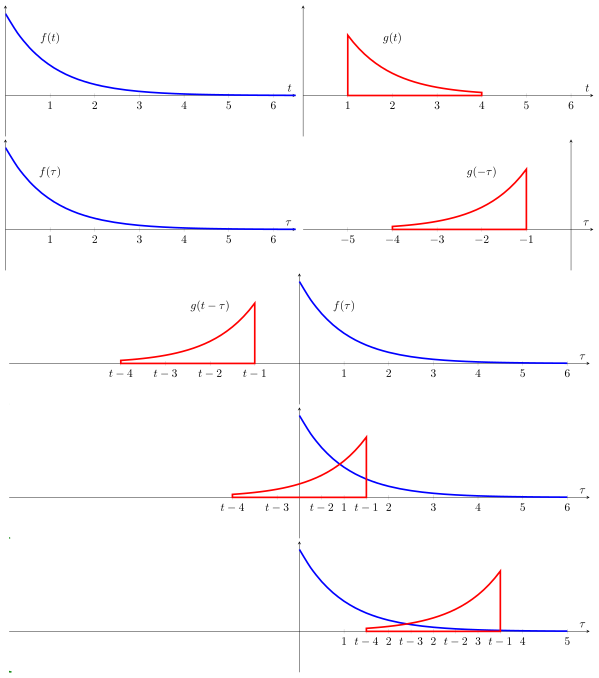
\includegraphics[width=0.4\textwidth]{08/convolution-steps}
    \caption{Operative illustration of convolution.}
\end{figure}

In the following example, we have a red-colored ``pulse'', $g(\tau)$, and a blue-colored pulse $f(\tau)$. The amount of yellow is the area of the product $f(\tau )\cdot g(t-\tau )$, computed by the convolution integral. The animation is created by continuously changing $t$ and recomputing the integral. The result (shown in black) is a function of $t$, not of $\tau$, but is plotted on the same axis as $\tau$, for convenience and comparison.

\begin{figure}[H]
    \centering
    \animategraphics[loop, autoplay, loop, width=0.7\textwidth]{20}{08/animations/convolution/convolution-}{0}{300}
    \caption{Convolution of two identical ``pulse'' functions. If the animation is not displayed correctly, try to enable JavaScript in your PDF reader or use Adobe Reader which has the correct extensions already enabled.}
\end{figure}

\subsection{Properties} 
%!TEX root=../../../root.tex

Consider a linear map $T:V \to W$, a basis $v_1,\dots,v_n \in V$ and a basis $w_1,\dots,w_m\in W$.
{
The \emph{matrix} of $T$ in these bases is the $m\times n$ array of values in $\mathbb{R}$
%
\[
\mathbf{T} = \begin{pmatrix}
    T_{1,1} & \cdots & T_{1,n} \\
    \vdots & & \vdots\\
    T_{m,1} & \cdots & T_{m,n}
  \end{pmatrix}
\]
%
whose entries $T_{i,j}$ are defined by
%
\[
{\color{darkgreen}Tv_j} = {\color{red}T_{1,j}} w_1 + \cdots + {\color{red}T_{m,j}} w_m
\]
}%

{
Hence each column of $\mathbf{T}$ contains the {\color{red}linear combination coefficients} for the {\color{darkgreen}image via $T$ of a basis vector from $V$}
}

{
In other words, the matrix encodes {\color{darkgreen}how basis vectors are mapped}, and this is enough to map all other vectors in their span, since:
\[ Tv = T ( \sum_j \alpha_j v_j ) = \sum_j T(\alpha_j v_j) = \sum_j \alpha_j {\color{darkgreen}Tv_j} \]
}

The matrix is a \emph{representation} for a linear map, and it \emph{depends on the choice of bases}.
Suppose $v \in V$ is an arbitrary vector, while $v_1,\dots,v_n$ is a basis of $V$. The matrix of $v$ wrt this basis is the $n\times 1$ matrix:
%
\[
\mathbf{v} = \begin{pmatrix}
    c_1 \\
    \vdots\\
    c_n
  \end{pmatrix}
\]
%
so that
%
\[
v = c_1 v_1 + \cdots c_n v_n
\]

Once again, we see that the matrix \emph{depends on the choice of basis} for $V$


\begin{itemize}
\item \textbf{addition}:  the matrix of $S+T$ can be obtained by summing the matrices of $S$ and $T${; this only makes sense if the \emph{same bases} are used for $S$, $T$, and $S+T$}
\item \textbf{scalar multiplication}: given $\lambda\in\mathbb{R}$, the matrix for $\lambda T$ is given by $\lambda$ times the matrix of $T$
\end{itemize}

{
In fact, we have just shown that \emph{matrices form a vector space} (Q1: what is the additive identity?) {(Q2: what is the vector space dimension?)}
}

{
We call $\mathbb{R}^{m\times n}$ the vector space of all $m\times n$ matrices with values in $\mathbb{R}$
}

{
\begin{itemize}
\item \textbf{product}: the matrix for $ST$ can be computed by the \emph{matrix product} between $\mathbf{S}$ and $\mathbf{T}$; in fact, the matrix product is defined precisely to make this work

{
Q3: is matrix product commutative?
}

{
Q4: do we need the same bases for $S:U\to V$ and $T:V \to W$?
}

\end{itemize}
}



Consider a linear map $T:V \to W$, a basis $v_1,\dots,v_n \in V$ and a basis $w_1,\dots,w_m\in W$.

%\medskip
%The $k$-th column of $\mathbf{T}$ equals the matrix vector $\mathbf{v}_k$:

%figure

From the definition of matrix product, one can show that it operates on a vector matrix as expected:
\[
\mathbf{Tv} =\mathbf{w} \quad \Leftrightarrow \quad Tv=w
\]
where $\mathbf{Tv}$ is the matrix product of $\mathbf{T}$ and $\mathbf{v}$, while $Tv$ simply denotes the function evaluation $T(v)$


{
\textbf{Remember:} $\mathbf{T}, \mathbf{v}, \mathbf{w}$ must follow a coherent choice of bases in order for the above to make sense. $\mathbf{v}$ can not be expressed in basis $\color{red}(\tilde{v}_1,\dots,\tilde{v}_n)$ if $\mathbf{T}$ only knows how to map basis vectors $\color{blue}({v}_1,\dots,{v}_n)$.
%
\[
T{\color{blue}v_j} = {\color{blue}T_{1,j}} w_1 + \cdots + {\color{blue}T_{m,j}} w_m
\]
%
%\[ Tv =  \sum_j \alpha_j T{\color{red}\tilde{v}_j} \]
}


\[
\underbrace{
\begin{pmatrix}
    T_{1,1} & \cdots & T_{1,n} \\
    \vdots & & \vdots\\
    T_{m,1} & \cdots & T_{m,n}
  \end{pmatrix}}_{\mathbf{T}}
  %
  \underbrace{
  \begin{pmatrix}
    c_1 \\
    \vdots \\
    c_n
  \end{pmatrix}}_{\mathbf{c}} =
  %
   \sum_{j=1}^n c_j \hspace{-0.6cm}
   \underbrace{\begin{pmatrix}
    {\color{red}T_{1,j}}  \\
    \vdots \\
    {\color{red}T_{m,j}}
  \end{pmatrix}}_{\mathrm{Tv_j~wrt~(w_1,\dots,w_m)}}
\]
%
\smallskip

Because recall that, for bases $v_1,\dots,v_n \in V$ and $w_1,\dots,w_m\in W$:
%
\[
Tv_j = {\color{red}T_{1,j}} w_1 + \cdots + {\color{red}T_{m,j}} w_m
\]

{
We see then that vector $c=\sum_j c_j v_j$ is mapped to $Tc = \sum_j c_j Tv_j$.

In other words, matrix product is behaving as expected.
}








\subsection{Discrete Convolution} 
%!TEX root=../../../root.tex

Consider a linear map $T:V \to W$, a basis $v_1,\dots,v_n \in V$ and a basis $w_1,\dots,w_m\in W$.
{
The \emph{matrix} of $T$ in these bases is the $m\times n$ array of values in $\mathbb{R}$
%
\[
\mathbf{T} = \begin{pmatrix}
    T_{1,1} & \cdots & T_{1,n} \\
    \vdots & & \vdots\\
    T_{m,1} & \cdots & T_{m,n}
  \end{pmatrix}
\]
%
whose entries $T_{i,j}$ are defined by
%
\[
{\color{darkgreen}Tv_j} = {\color{red}T_{1,j}} w_1 + \cdots + {\color{red}T_{m,j}} w_m
\]
}%

{
Hence each column of $\mathbf{T}$ contains the {\color{red}linear combination coefficients} for the {\color{darkgreen}image via $T$ of a basis vector from $V$}
}

{
In other words, the matrix encodes {\color{darkgreen}how basis vectors are mapped}, and this is enough to map all other vectors in their span, since:
\[ Tv = T ( \sum_j \alpha_j v_j ) = \sum_j T(\alpha_j v_j) = \sum_j \alpha_j {\color{darkgreen}Tv_j} \]
}

The matrix is a \emph{representation} for a linear map, and it \emph{depends on the choice of bases}.
Suppose $v \in V$ is an arbitrary vector, while $v_1,\dots,v_n$ is a basis of $V$. The matrix of $v$ wrt this basis is the $n\times 1$ matrix:
%
\[
\mathbf{v} = \begin{pmatrix}
    c_1 \\
    \vdots\\
    c_n
  \end{pmatrix}
\]
%
so that
%
\[
v = c_1 v_1 + \cdots c_n v_n
\]

Once again, we see that the matrix \emph{depends on the choice of basis} for $V$


\begin{itemize}
\item \textbf{addition}:  the matrix of $S+T$ can be obtained by summing the matrices of $S$ and $T${; this only makes sense if the \emph{same bases} are used for $S$, $T$, and $S+T$}
\item \textbf{scalar multiplication}: given $\lambda\in\mathbb{R}$, the matrix for $\lambda T$ is given by $\lambda$ times the matrix of $T$
\end{itemize}

{
In fact, we have just shown that \emph{matrices form a vector space} (Q1: what is the additive identity?) {(Q2: what is the vector space dimension?)}
}

{
We call $\mathbb{R}^{m\times n}$ the vector space of all $m\times n$ matrices with values in $\mathbb{R}$
}

{
\begin{itemize}
\item \textbf{product}: the matrix for $ST$ can be computed by the \emph{matrix product} between $\mathbf{S}$ and $\mathbf{T}$; in fact, the matrix product is defined precisely to make this work

{
Q3: is matrix product commutative?
}

{
Q4: do we need the same bases for $S:U\to V$ and $T:V \to W$?
}

\end{itemize}
}



Consider a linear map $T:V \to W$, a basis $v_1,\dots,v_n \in V$ and a basis $w_1,\dots,w_m\in W$.

%\medskip
%The $k$-th column of $\mathbf{T}$ equals the matrix vector $\mathbf{v}_k$:

%figure

From the definition of matrix product, one can show that it operates on a vector matrix as expected:
\[
\mathbf{Tv} =\mathbf{w} \quad \Leftrightarrow \quad Tv=w
\]
where $\mathbf{Tv}$ is the matrix product of $\mathbf{T}$ and $\mathbf{v}$, while $Tv$ simply denotes the function evaluation $T(v)$


{
\textbf{Remember:} $\mathbf{T}, \mathbf{v}, \mathbf{w}$ must follow a coherent choice of bases in order for the above to make sense. $\mathbf{v}$ can not be expressed in basis $\color{red}(\tilde{v}_1,\dots,\tilde{v}_n)$ if $\mathbf{T}$ only knows how to map basis vectors $\color{blue}({v}_1,\dots,{v}_n)$.
%
\[
T{\color{blue}v_j} = {\color{blue}T_{1,j}} w_1 + \cdots + {\color{blue}T_{m,j}} w_m
\]
%
%\[ Tv =  \sum_j \alpha_j T{\color{red}\tilde{v}_j} \]
}


\[
\underbrace{
\begin{pmatrix}
    T_{1,1} & \cdots & T_{1,n} \\
    \vdots & & \vdots\\
    T_{m,1} & \cdots & T_{m,n}
  \end{pmatrix}}_{\mathbf{T}}
  %
  \underbrace{
  \begin{pmatrix}
    c_1 \\
    \vdots \\
    c_n
  \end{pmatrix}}_{\mathbf{c}} =
  %
   \sum_{j=1}^n c_j \hspace{-0.6cm}
   \underbrace{\begin{pmatrix}
    {\color{red}T_{1,j}}  \\
    \vdots \\
    {\color{red}T_{m,j}}
  \end{pmatrix}}_{\mathrm{Tv_j~wrt~(w_1,\dots,w_m)}}
\]
%
\smallskip

Because recall that, for bases $v_1,\dots,v_n \in V$ and $w_1,\dots,w_m\in W$:
%
\[
Tv_j = {\color{red}T_{1,j}} w_1 + \cdots + {\color{red}T_{m,j}} w_m
\]

{
We see then that vector $c=\sum_j c_j v_j$ is mapped to $Tc = \sum_j c_j Tv_j$.

In other words, matrix product is behaving as expected.
}








